\documentclass{standalone}
\usepackage{tikz}
\usetikzlibrary{patterns, positioning}


\begin{document}
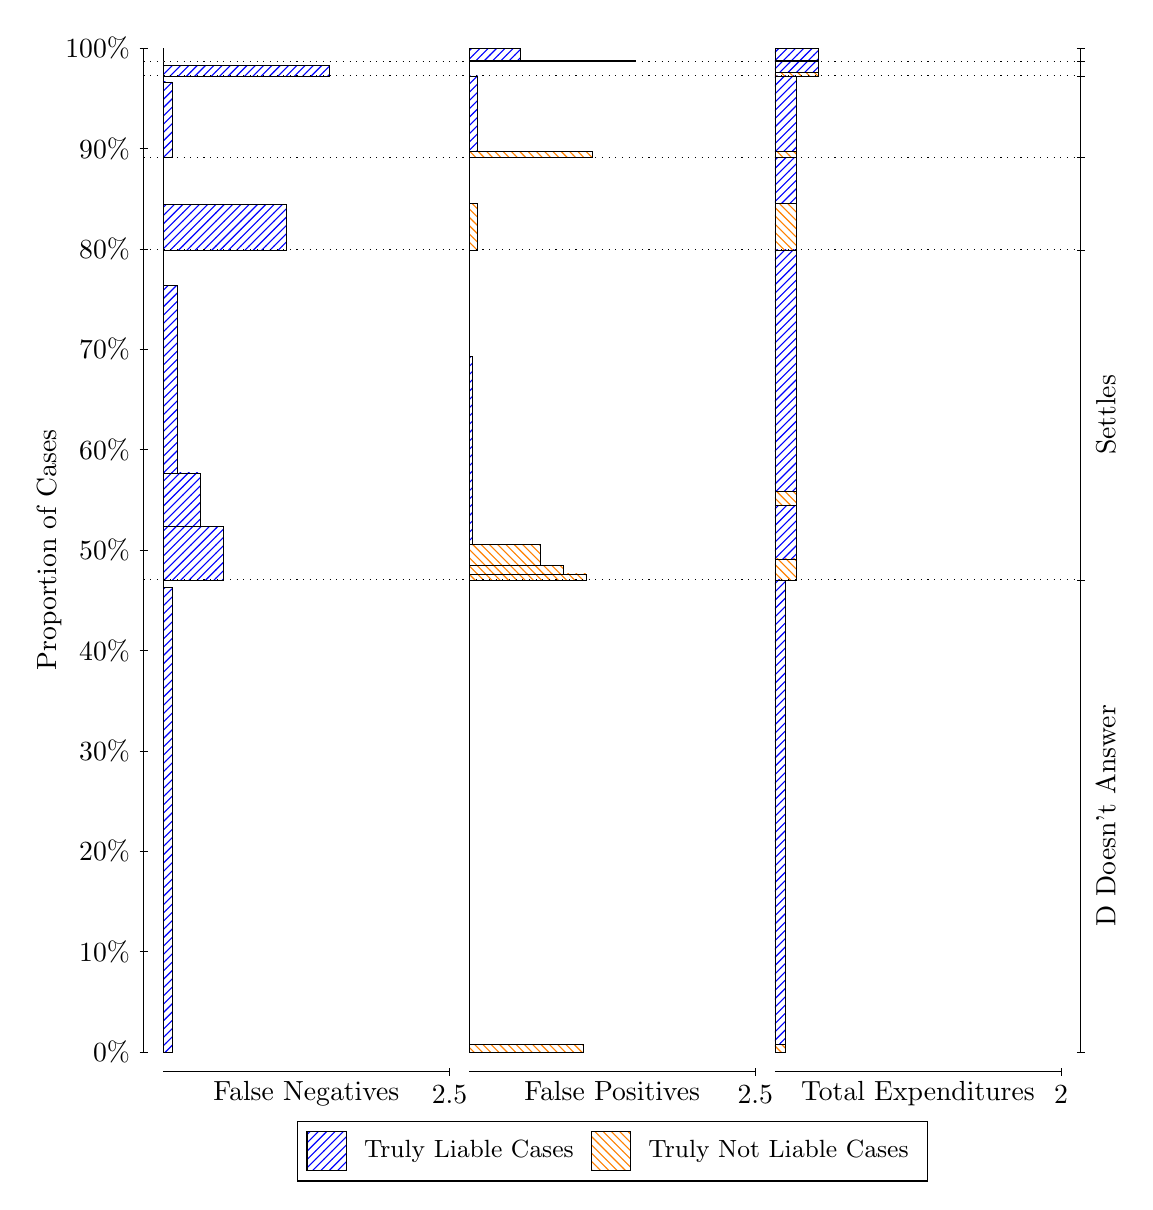
\begin{tikzpicture}
\draw[black, very thin] (1.5,1.75) -- (1.5,14.5);
\node[rotate=90, text=black, anchor=center] at (0.3, 8.125) {Proportion of Cases};
\draw[black, very thin] (1.45,1.75) -- (1.55,1.75);
\node[text=black, anchor=east] at (1.45, 1.75) {0\%};
\draw[black, very thin] (1.45,3.025) -- (1.55,3.025);
\node[text=black, anchor=east] at (1.45, 3.025) {10\%};
\draw[black, very thin] (1.45,4.3) -- (1.55,4.3);
\node[text=black, anchor=east] at (1.45, 4.3) {20\%};
\draw[black, very thin] (1.45,5.575) -- (1.55,5.575);
\node[text=black, anchor=east] at (1.45, 5.575) {30\%};
\draw[black, very thin] (1.45,6.85) -- (1.55,6.85);
\node[text=black, anchor=east] at (1.45, 6.85) {40\%};
\draw[black, very thin] (1.45,8.125) -- (1.55,8.125);
\node[text=black, anchor=east] at (1.45, 8.125) {50\%};
\draw[black, very thin] (1.45,9.4) -- (1.55,9.4);
\node[text=black, anchor=east] at (1.45, 9.4) {60\%};
\draw[black, very thin] (1.45,10.675) -- (1.55,10.675);
\node[text=black, anchor=east] at (1.45, 10.675) {70\%};
\draw[black, very thin] (1.45,11.95) -- (1.55,11.95);
\node[text=black, anchor=east] at (1.45, 11.95) {80\%};
\draw[black, very thin] (1.45,13.225) -- (1.55,13.225);
\node[text=black, anchor=east] at (1.45, 13.225) {90\%};
\draw[black, very thin] (1.45,14.5) -- (1.55,14.5);
\node[text=black, anchor=east] at (1.45, 14.5) {100\%};

\draw[black, very thin] (13.4,1.75) -- (13.4,14.5);
\draw[black, very thin] (13.35,1.75) -- (13.45,1.75);
\node[anchor=west] at (13.35, 1.75) {};
\draw[black, very thin] (13.35,7.7461) -- (13.45,7.7461);
\node[anchor=west] at (13.35, 7.7461) {};
\draw[black, very thin] (13.35,11.936) -- (13.45,11.936);
\node[anchor=west] at (13.35, 11.936) {};
\draw[black, very thin] (13.35,13.109) -- (13.45,13.109);
\node[anchor=west] at (13.35, 13.109) {};
\draw[black, very thin] (13.35,14.146) -- (13.45,14.146);
\node[anchor=west] at (13.35, 14.146) {};
\draw[black, very thin] (13.35,14.332) -- (13.45,14.332);
\node[anchor=west] at (13.35, 14.332) {};
\draw[black, very thin] (13.35,14.5) -- (13.45,14.5);
\node[anchor=west] at (13.35, 14.5) {};

\draw[black, very thin, pattern color=blue, pattern=north east lines] (1.75,1.75) rectangle (1.859,7.6492);
\draw[black, very thin, pattern color=orange, pattern=north west lines] (1.75,7.6492) rectangle (1.75,7.7461);
\draw[black, very thin, pattern color=blue, pattern=north east lines] (1.75,7.7461) rectangle (2.513,8.4242);
\draw[black, very thin, pattern color=blue, pattern=north east lines] (1.75,8.4242) rectangle (2.2223,9.1031);
\draw[black, very thin, pattern color=blue, pattern=north east lines] (1.75,9.1031) rectangle (1.9317,11.489);
\draw[black, very thin, pattern color=orange, pattern=north west lines] (1.75,11.489) rectangle (1.75,11.936);
\draw[black, very thin, pattern color=blue, pattern=north east lines] (1.75,11.936) rectangle (3.3123,12.518);
\draw[black, very thin, pattern color=orange, pattern=north west lines] (1.75,12.518) rectangle (1.75,13.109);
\draw[black, very thin, pattern color=blue, pattern=north east lines] (1.75,13.109) rectangle (1.859,14.071);
\draw[black, very thin, pattern color=orange, pattern=north west lines] (1.75,14.071) rectangle (1.75,14.146);
\draw[black, very thin, pattern color=blue, pattern=north east lines] (1.75,14.146) rectangle (3.8573,14.284);
\draw[black, very thin, pattern color=orange, pattern=north west lines] (1.75,14.284) rectangle (1.75,14.332);
\draw[black, very thin, pattern color=orange, pattern=north west lines] (1.75,14.332) rectangle (1.75,14.347);
\draw[black, very thin, pattern color=blue, pattern=north east lines] (1.75,14.347) rectangle (1.75,14.5);
\draw[black, very thin, pattern color=orange, pattern=north west lines] (5.6333,1.75) rectangle (7.0867,1.8469);
\draw[black, very thin, pattern color=blue, pattern=north east lines] (5.6333,1.8469) rectangle (5.6333,7.7461);
\draw[black, very thin, pattern color=orange, pattern=north west lines] (5.6333,7.7461) rectangle (7.123,7.8214);
\draw[black, very thin, pattern color=orange, pattern=north west lines] (5.6333,7.8214) rectangle (6.8323,7.9282);
\draw[black, very thin, pattern color=orange, pattern=north west lines] (5.6333,7.9282) rectangle (6.5417,8.1933);
\draw[black, very thin, pattern color=blue, pattern=north east lines] (5.6333,8.1933) rectangle (5.6697,10.579);
\draw[black, very thin, pattern color=blue, pattern=north east lines] (5.6333,10.579) rectangle (5.6333,11.936);
\draw[black, very thin, pattern color=orange, pattern=north west lines] (5.6333,11.936) rectangle (5.7423,12.528);
\draw[black, very thin, pattern color=blue, pattern=north east lines] (5.6333,12.528) rectangle (5.6333,13.109);
\draw[black, very thin, pattern color=orange, pattern=north west lines] (5.6333,13.109) rectangle (7.1957,13.185);
\draw[black, very thin, pattern color=blue, pattern=north east lines] (5.6333,13.185) rectangle (5.7423,14.146);
\draw[black, very thin, pattern color=orange, pattern=north west lines] (5.6333,14.146) rectangle (5.6333,14.194);
\draw[black, very thin, pattern color=blue, pattern=north east lines] (5.6333,14.194) rectangle (5.6333,14.332);
\draw[black, very thin, pattern color=orange, pattern=north west lines] (5.6333,14.332) rectangle (7.7407,14.347);
\draw[black, very thin, pattern color=blue, pattern=north east lines] (5.6333,14.347) rectangle (6.2873,14.5);
\draw[black, very thin, pattern color=orange, pattern=north west lines] (9.5167,1.75) rectangle (9.6529,1.8469);
\draw[black, very thin, pattern color=blue, pattern=north east lines] (9.5167,1.8469) rectangle (9.6529,7.7461);
\draw[black, very thin, pattern color=orange, pattern=north west lines] (9.5167,7.7461) rectangle (9.7892,8.0112);
\draw[black, very thin, pattern color=blue, pattern=north east lines] (9.5167,8.0112) rectangle (9.7892,8.6893);
\draw[black, very thin, pattern color=orange, pattern=north west lines] (9.5167,8.6893) rectangle (9.7892,8.8714);
\draw[black, very thin, pattern color=blue, pattern=north east lines] (9.5167,8.8714) rectangle (9.7892,11.936);
\draw[black, very thin, pattern color=orange, pattern=north west lines] (9.5167,11.936) rectangle (9.7892,12.528);
\draw[black, very thin, pattern color=blue, pattern=north east lines] (9.5167,12.528) rectangle (9.7892,13.109);
\draw[black, very thin, pattern color=orange, pattern=north west lines] (9.5167,13.109) rectangle (9.7892,13.185);
\draw[black, very thin, pattern color=blue, pattern=north east lines] (9.5167,13.185) rectangle (9.7892,14.146);
\draw[black, very thin, pattern color=orange, pattern=north west lines] (9.5167,14.146) rectangle (10.062,14.194);
\draw[black, very thin, pattern color=blue, pattern=north east lines] (9.5167,14.194) rectangle (10.062,14.332);
\draw[black, very thin, pattern color=orange, pattern=north west lines] (9.5167,14.332) rectangle (10.062,14.347);
\draw[black, very thin, pattern color=blue, pattern=north east lines] (9.5167,14.347) rectangle (10.062,14.5);
\draw[black, dotted] (1.5,7.7461) -- (13.4,7.7461);
\draw[black, dotted] (1.5,11.936) -- (13.4,11.936);
\draw[black, dotted] (1.5,13.109) -- (13.4,13.109);
\draw[black, dotted] (1.5,14.146) -- (13.4,14.146);
\draw[black, dotted] (1.5,14.332) -- (13.4,14.332);
\draw[black, very thin] (1.75,1.5) -- (5.3833,1.5);
\node[text=black, anchor=north] at (3.5667, 1.5) {False Negatives};
\draw[black, very thin] (5.3833,1.45) -- (5.3833,1.55);
\node[text=black, anchor=north] at (5.3833, 1.45) {2.5};

\draw[black, very thin] (5.6333,1.5) -- (9.2667,1.5);
\node[text=black, anchor=north] at (7.45, 1.5) {False Positives};
\draw[black, very thin] (9.2667,1.45) -- (9.2667,1.55);
\node[text=black, anchor=north] at (9.2667, 1.45) {2.5};

\draw[black, very thin] (9.5167,1.5) -- (13.15,1.5);
\node[text=black, anchor=north] at (11.333, 1.5) {Total Expenditures};
\draw[black, very thin] (13.15,1.45) -- (13.15,1.55);
\node[text=black, anchor=north] at (13.15, 1.45) {2};

\node[text=black, centered, rotate=90] at (13.72, 4.748) {D Doesn't Answer};
\node[text=black, centered, rotate=90] at (13.72, 9.841) {Settles};





\draw (7.449999999999999,1.5) node[draw=none] (baseCoordinate) {};
\begin{scope}[align=center]
        \matrix[scale=0.5, draw=black, below=0.5cm of baseCoordinate, nodes={draw}, column sep=0.1cm]{
            \node[rectangle, draw, minimum width=0.5cm, minimum height=0.5cm, pattern color=blue, pattern=north east lines] {}; &
            \node[draw=none, font=\small, text=black] (B) {Truly Liable Cases}; &
            \node[rectangle, draw, minimum width=0.5cm, minimum height=0.5cm, pattern color=orange, pattern=north west lines] {}; &
            \node[draw=none, font=\small, text=black] (B) {Truly Not Liable Cases}; \\
            };
\end{scope}

\end{tikzpicture}
\end{document}